\documentclass[8pt,landscape]{article}
\usepackage[landscape,margin=0.3in]{geometry}
\usepackage{multicol}
\usepackage{amsmath}
\usepackage{amssymb}
\usepackage{enumitem}
\usepackage{xcolor}
\usepackage{tikz}
\usepackage{pgfplots}
\pgfplotsset{compat=1.18}
\usetikzlibrary{arrows.meta}

% Reduce spacing
\setlength{\parindent}{0pt}
\setlength{\parskip}{1pt}
\setlength{\columnsep}{12pt}
\setlist{nosep,leftmargin=8pt}

% Compact sections
\usepackage{titlesec}
\titleformat{\section}{\normalsize\bfseries\color{blue!70!black}}{\thesection}{0.3em}{}
\titlespacing*{\section}{0pt}{3pt}{1pt}
\titleformat{\subsection}{\small\bfseries\color{blue!50!black}}{\thesubsection}{0.3em}{}
\titlespacing*{\subsection}{0pt}{2pt}{1pt}

\newcommand{\formula}[2]{\textbf{#1:} $#2$}
\newcommand{\tip}[1]{\textcolor{red!70!black}{\textbf{!} #1}}

\begin{document}
\begin{multicols}{4}
\tiny

\begin{center}
\large\textbf{ECO310 Midterm Cheat Sheet}
\end{center}

\section{Preferences \& Utility}

\textbf{Rational:} Complete + Transitive

\textbf{Monotone:} More is better

\textbf{Convex:} Mixtures $\geq$ extremes (ICs bow inward)

\subsection{MRS}
$$MRS = \frac{MU_1}{MU_2} = -\frac{dx_2}{dx_1}\bigg|_{IC}$$

At optimum: $MRS = p_1/p_2$

\begin{center}
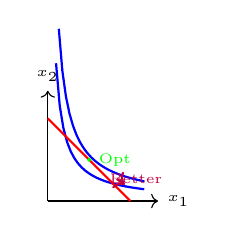
\begin{tikzpicture}[scale=0.35]
\draw[->] (0,0) -- (4,0) node[right] {\tiny $x_1$};
\draw[->] (0,0) -- (0,4) node[above] {\tiny $x_2$};
\draw[blue,thick] plot[domain=0.3:3.5] (\x,{1.5/\x});
\draw[blue,thick] plot[domain=0.4:3.5] (\x,{2.5/\x});
\draw[red,thick] (0,3) -- (3,0);
\filldraw[green] (1.5,1.5) circle (1.5pt);
\node[green,right] at (1.5,1.5) {\tiny Opt};
\draw[->,purple,thick] (2.5,0.8) -- (2.8,0.6);
\node[purple] at (3.2,0.8) {\tiny Better};
\end{tikzpicture}
\end{center}

\subsection{Budget Constraint}
$$p_1 x_1 + p_2 x_2 = m$$

Slope: $-p_1/p_2$, Intercepts: $(m/p_1, 0)$, $(0, m/p_2)$

\section{Utility Functions}

\subsection{Cobb-Douglas}
$$u = x_1^a x_2^b$$

\tip{Magic Rule:} Spend $\frac{a}{a+b}$ on good 1, $\frac{b}{a+b}$ on good 2

$$x_1^* = \frac{a}{a+b} \cdot \frac{m}{p_1}, \quad x_2^* = \frac{b}{a+b} \cdot \frac{m}{p_2}$$

$MRS = \frac{a}{b} \cdot \frac{x_2}{x_1}$

\subsection{Perfect Complements}
$$u = \min\{ax_1, bx_2\}$$

Always at kink: $ax_1 = bx_2$

$$x_1^* = \frac{bm}{bp_1 + ap_2}, \quad x_2^* = \frac{am}{bp_1 + ap_2}$$

\tip{No substitution effect!} (only income effect)

\begin{center}
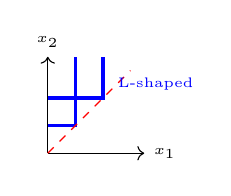
\begin{tikzpicture}[scale=0.35]
\draw[->] (0,0) -- (3.5,0) node[right] {\tiny $x_1$};
\draw[->] (0,0) -- (0,3.5) node[above] {\tiny $x_2$};
\draw[blue,very thick] (0,1) -- (1,1) -- (1,3.5);
\draw[blue,very thick] (0,2) -- (2,2) -- (2,3.5);
\draw[red,dashed] (0,0) -- (3,3);
\node[blue,right] at (2.2,2.5) {\tiny L-shaped};
\end{tikzpicture}
\end{center}

\subsection{Perfect Substitutes}
$$u = ax_1 + bx_2$$

$MRS = -a/b$ (constant)

\tip{Buy all of cheaper good:}
\begin{itemize}
    \item If $\frac{a}{p_1} > \frac{b}{p_2}$: $x_1 = m/p_1$, $x_2 = 0$
    \item If $\frac{a}{p_1} < \frac{b}{p_2}$: $x_1 = 0$, $x_2 = m/p_2$
\end{itemize}

\subsection{Quasilinear}
$$u = v(x_1) + x_2$$

$MRS = v'(x_1)$ (only depends on $x_1$)

\tip{No income effect for $x_1$} (at interior)

\subsection{CES}
$$u = (x_1^r + x_2^r)^{1/r}$$

$r \to 0$: CD; $r \to -\infty$: PC; $r = 1$: PS

\section{Optimal Choice}

\subsection{Interior Solution}
\textbf{Tangency:} $\frac{MU_1}{p_1} = \frac{MU_2}{p_2}$ or $MRS = \frac{p_1}{p_2}$

\textbf{Budget:} $p_1 x_1 + p_2 x_2 = m$

Solve both equations for $x_1^*, x_2^*$

\subsection{Lagrangian}
$$\mathcal{L} = u(x_1, x_2) + \lambda[m - p_1 x_1 - p_2 x_2]$$

FOCs: $MU_i = \lambda p_i$ for each $i$

$\lambda$ = marginal utility of income

\subsection{Corner Solution}
Check: $x_i \geq 0$ always!

If $MRS > p_1/p_2$ everywhere: buy only $x_1$

If $MRS < p_1/p_2$ everywhere: buy only $x_2$

\section{Income \& Sub Effects}

\textbf{Total = Substitution + Income}

\begin{center}
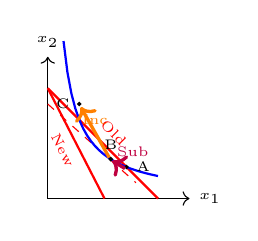
\begin{tikzpicture}[scale=0.4]
\draw[->] (0,0) -- (4.5,0) node[right] {\tiny $x_1$};
\draw[->] (0,0) -- (0,4.5) node[above] {\tiny $x_2$};
\draw[red,thick] (0,3.5) -- (3.5,0) node[midway,above,sloped] {\tiny Old};
\draw[red,thick] (0,3.5) -- (1.8,0) node[midway,below,sloped] {\tiny New};
\draw[red,dashed] (0,3) -- (2.8,0.5);
\draw[blue,thick] plot[domain=0.5:3.5] (\x,{2.5/\x});
\filldraw (2.5,1) circle (1.5pt) node[right] {\tiny A};
\filldraw (2,1.25) circle (1.5pt) node[above] {\tiny B};
\filldraw (1,3) circle (1.5pt) node[left] {\tiny C};
\draw[->,purple,very thick] (2.45,0.95) -- (2.05,1.2);
\node[purple] at (2.7,1.5) {\tiny Sub};
\draw[->,orange,very thick] (1.95,1.3) -- (1.05,2.9);
\node[orange] at (1.5,2.5) {\tiny Inc};
\end{tikzpicture}
\end{center}

\textbf{Sub effect:} Always $\leq 0$ (buy less when $p$ rises)
- Move along IC to new price ratio
- $=$ compensated bundle $-$ original

\textbf{Income effect:} Sign depends on normal/inferior
- Normal: $< 0$ (buy less)
- Inferior: $> 0$ (buy more)
- $=$ new bundle $-$ compensated

\tip{Giffen:} Income effect dominates, demand increases when price rises

\section{Uncertainty}

\subsection{Expected Utility}
$$EU(L) = \sum p_i u(c_i)$$

\textbf{vNM utility:} Unique up to $\tilde{u} = a + bu$ ($b > 0$)

\tip{NOT arbitrary transforms!}

\subsection{Risk Aversion}
$$u'' < 0 \Leftrightarrow \text{Risk Averse}$$

Prefer certainty to gambles: $u(E[x]) > E[u(x)]$

\begin{center}
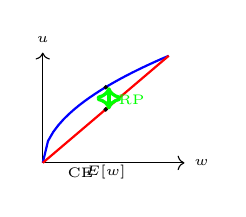
\begin{tikzpicture}[scale=0.4]
\draw[->] (0,0) -- (4.5,0) node[right] {\tiny $w$};
\draw[->] (0,0) -- (0,3.5) node[above] {\tiny $u$};
\draw[blue,thick,domain=0:4] plot (\x,{1.7*sqrt(\x)});
\draw[red,thick] (0,0) -- (4,3.4);
\filldraw (2,2.4) circle (1.5pt);
\filldraw (2,1.7) circle (1.5pt);
\draw[<->,green,very thick] (2.1,1.7) -- (2.1,2.4);
\node[green,right] at (2.1,2) {\tiny RP};
\node at (2,-0.3) {\tiny $E[w]$};
\node at (1.2,-0.3) {\tiny CE};
\end{tikzpicture}
\end{center}

\textbf{CE:} $u(CE) = EU$

\textbf{RP:} $RP = E[w] - CE$ (how much pay to avoid risk)

Risk averse: $RP > 0$

\subsection{Arrow-Pratt}
$$r_A(x) = -\frac{u''(x)}{u'(x)}, \quad r_R(x) = x \cdot r_A(x)$$

Higher $r_A$ $\Rightarrow$ more risk averse

\textbf{CRRA:} $u = \frac{x^{1-\rho}}{1-\rho}$ or $\ln x$
- $r_A = \rho/x$ (DARA), $r_R = \rho$

\textbf{CARA:} $u = -e^{-\alpha x}$
- $r_A = \alpha$, $r_R = \alpha x$ (IRRA)

\subsection{Insurance}
Wealth $w$, loss $D$ prob $\pi$, premium $q$, coverage $K$

$$EU = (1-\pi)u(w-qK) + \pi u(w-D+K(1-q))$$

\textbf{Fair:} $q = \pi$ $\Rightarrow$ full insurance ($K = D$)

\textbf{Unfair:} $q > \pi$ $\Rightarrow$ partial insurance ($K < D$)

FOC: $(1-\pi)u'(c_1)(-q) + \pi u'(c_2)(1-q) = 0$

\subsection{Portfolio}
Invest $a$ in risky (return $\tilde{r}$), rest at $r_f$:

$$\tilde{W} = w(1 + r_f) + a(\tilde{r} - r_f)$$

FOC: $E[u'(\tilde{W})(\tilde{r} - r_f)] = 0$

If $E[\tilde{r}] > r_f$: invest $a^* > 0$

\section{General Equilibrium}

\subsection{Edgeworth Box}
2 consumers, 2 goods, total $(E_1, E_2)$

\begin{center}
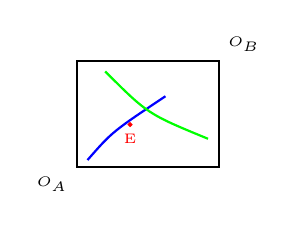
\begin{tikzpicture}[scale=0.45]
\draw[thick] (0,0) rectangle (4,3);
\node[below left] at (0,0) {\tiny $O_A$};
\node[above right] at (4,3) {\tiny $O_B$};
\draw[blue,thick] (0.3,0.2) .. controls (1,1) .. (2.5,2);
\draw[green,thick] (0.8,2.7) .. controls (2,1.5) .. (3.7,0.8);
\filldraw[red] (1.5,1.2) circle (1.5pt);
\node[red,below] at (1.5,1.2) {\tiny E};
\end{tikzpicture}
\end{center}

\textbf{Feasible:} $x^A + x^B = E$

\textbf{PE:} $MRS^A = MRS^B$ (ICs tangent)

\subsection{Competitive Equilibrium}
Each: $\max u$ s.t. $p \cdot x = p \cdot e$ (endowment)

Markets clear: $\sum x_i = E_i$

\textbf{Walras' Law:} If $n-1$ markets clear, $n$-th clears

\textbf{How to solve:}
\begin{enumerate}
    \item Set $p_2 = 1$ (numeraire)
    \item Income: $m^i = p_1 e_1^i + e_2^i$
    \item Demands: $x_1^i(p_1)$ from each UMP
    \item Market clear: $\sum x_1^i(p_1) = E_1$
    \item Solve for $p_1^*$
\end{enumerate}

\subsection{Welfare Theorems}
\textbf{1st:} CE $\Rightarrow$ PE (needs LNS)

\textbf{2nd:} Any PE can be CE with transfers (needs convexity)

\section{Duality}

\subsection{Expenditure Function}
$$e(p, \bar{u}) = \min p \cdot x \text{ s.t. } u(x) \geq \bar{u}$$

Gives Hicksian demand: $h_i(p, \bar{u})$

\textbf{Shepard's Lemma:} $h_i = \frac{\partial e}{\partial p_i}$

\subsection{Relations}
$$x_i(p, m) = h_i(p, v(p, m))$$
$$h_i(p, \bar{u}) = x_i(p, e(p, \bar{u}))$$
$$v(p, e(p, \bar{u})) = \bar{u}$$
$$e(p, v(p, m)) = m$$

\section{WARP}

If $x$ chosen when $y$ affordable, and $y$ chosen later, then $y$ must NOT have been affordable when $x$ chosen.

\textbf{Check:} For $(p^A, m^A)$ and $(p^B, m^B)$:
\begin{itemize}
    \item Is $p^B \cdot x^A \leq m^B$?
    \item Is $p^A \cdot x^B \leq m^A$?
    \item If both strictly: WARP violation
\end{itemize}

$\alpha + \beta \Leftrightarrow$ Rationalizable $\Leftrightarrow$ WARP

\section{Quick Tips}

\tip{Always check $x_i \geq 0$!}

\tip{CD:} Use fraction rule, don't solve manually

\tip{PC:} Zero sub effect, all income

\tip{PS:} Corner solution (all or nothing)

\tip{QL:} No income effect for $x_1$

\tip{vNM:} Only affine transforms allowed

\tip{Sub effect:} Always negative for own price

\tip{Giffen:} Rare - income dominates sub

\tip{Risk averse:} Concave $u$, $u'' < 0$

\tip{Fair insurance:} Full coverage optimal

\tip{PE:} $MRS^A = MRS^B$ at tangency

\tip{Walras:} Only need $n-1$ market clearing

\columnbreak

\section{Problem Templates}

\subsection{UMP with CD}
Given: $u = x_1^a x_2^b$, $(p_1, p_2, m)$

\textbf{Solution:}
$$x_1^* = \frac{a}{a+b} \cdot \frac{m}{p_1}, \quad x_2^* = \frac{b}{a+b} \cdot \frac{m}{p_2}$$

Done! (No calculus needed)

\subsection{UMP General}
1. $MRS = MU_1/MU_2$

2. Set $MRS = p_1/p_2$

3. Solve for $x_2(x_1)$ or $x_1(x_2)$

4. Plug into $p_1 x_1 + p_2 x_2 = m$

5. Solve for $x_1^*$, $x_2^*$

6. Check: both $\geq 0$?

\subsection{Income/Sub Effects}
When $p_1$ changes from $p_1$ to $p_1'$:

1. \textbf{Original:} $A = (x_1, x_2)$ at $(p_1, p_2, m)$

2. \textbf{Utility:} $\bar{u} = u(A)$

3. \textbf{Compensated:} Solve $\min p_1' x_1 + p_2 x_2$ s.t. $u(x) = \bar{u}$

   Get $B = (x_1^c, x_2^c)$

4. \textbf{New:} $C = (x_1', x_2')$ at $(p_1', p_2, m)$

5. Sub $= B - A$, Income $= C - B$

\subsection{Expected Utility}
Given: States $s=1,\ldots,n$ with probs $p_s$, outcomes $c_s$, utility $u$

1. $EU = \sum_s p_s u(c_s)$

2. If choosing $x$: write $c_s(x)$, $EU(x) = \sum_s p_s u(c_s(x))$

3. FOC: $\frac{dEU}{dx} = \sum_s p_s u'(c_s) \frac{dc_s}{dx} = 0$

4. Solve for $x^*$

\subsection{CE and RP}
Given: Lottery with $EU$, utility $u$

1. Find $E[w] = \sum p_i w_i$

2. Find $EU = \sum p_i u(w_i)$

3. Solve $u(CE) = EU$ for $CE$

4. $RP = E[w] - CE$

\subsection{General Equilibrium}
Given: 2 consumers with utilities $u^A, u^B$, endowments $e^A, e^B$

1. Normalize $p_2 = 1$

2. Incomes: $m^A = p_1 e_1^A + e_2^A$, $m^B = p_1 e_1^B + e_2^B$

3. Solve UMPs: $x_1^A(p_1)$, $x_1^B(p_1)$

4. Market clear: $x_1^A(p_1) + x_1^B(p_1) = e_1^A + e_1^B$

5. Solve for $p_1^*$

6. Find allocations: $(x_1^A(p_1^*), x_2^A(p_1^*))$, etc.

7. Check: all $\geq 0$

\section{Common Mistakes}

\tip{Mixing up $x(p,m)$ vs $h(p,\bar{u})$}

\tip{Sub effect: direction!} (Less of good when price rises)

\tip{PC: no sub effect} (everything is income)

\tip{vNM: can't use $u^2$ or $\sqrt{u}$} (only $a+bu$)

\tip{Variance vs std dev} ($\sigma^2$ vs $\sigma$)

\tip{Corner: set $x=0$, don't use FOC}

\tip{"Spend \$X" $\neq$ "Buy X units"} (unless $p=1$)

\tip{Quasilinear: check $x_2 \geq 0$}

\tip{CE allocations: verify market clearing}

\tip{WARP: "revealed preferred" = chosen when other affordable}

\section{Key Formulas}

\subsection{Derivatives}
$\frac{d}{dx}(x^n) = nx^{n-1}$

$\frac{d}{dx}(\ln x) = \frac{1}{x}$

$\frac{d}{dx}(e^x) = e^x$

$\frac{d}{dx}(e^{ax}) = ae^{ax}$

\subsection{Algebra}
$x^a x^b = x^{a+b}$

$(x^a)^b = x^{ab}$

$\ln(xy) = \ln x + \ln y$

$\ln(x^a) = a \ln x$

$e^{\ln x} = x$, $\ln(e^x) = x$

\subsection{Optimization}
FOC: $\frac{df}{dx} = 0$

SOC: $\frac{d^2f}{dx^2} < 0$ (max), $> 0$ (min)

Constrained: Use Lagrangian

$$\mathcal{L} = f(x) + \lambda[g(x) - c]$$

FOC: $\frac{\partial \mathcal{L}}{\partial x} = 0$, $\frac{\partial \mathcal{L}}{\partial \lambda} = 0$

\subsection{Probability}
$E[X] = \sum_i p_i x_i$

$\text{Var}(X) = E[X^2] - (E[X])^2$

$\sigma = \sqrt{\text{Var}(X)}$

\section{Exam Strategy}

1. \textbf{Read carefully:} What type of utility?

2. \textbf{CD shortcut:} Don't waste time on calculus

3. \textbf{Check corners:} Always verify $x \geq 0$

4. \textbf{Draw diagrams:} ICs + budget for intuition

5. \textbf{Sub effect:} Always negative for own price

6. \textbf{State-contingent:} Label states clearly

7. \textbf{Units:} Match dimensions (dollars, utils, etc.)

8. \textbf{Final check:} Does answer make economic sense?

\end{multicols}
\end{document}
